% Created 2019-03-04 lun 14:09
\documentclass[11pt]{article}
\usepackage[utf8]{inputenc}
\usepackage[T1]{fontenc}
\usepackage[spanish]{babel}
\usepackage{caption}
\usepackage{fixltx2e}
\usepackage{graphicx}
\usepackage{longtable}
\usepackage{float}
\usepackage{wrapfig}
\usepackage{rotating}
\usepackage[normalem]{ulem}
\usepackage{amsmath}
\usepackage{textcomp}
\usepackage{marvosym}
\usepackage{wasysym}
\usepackage{amssymb}
\usepackage{hyperref}
\tolerance=1000
\author{Daniel Fernández Pérez\\Miguel García-Mauriño Taboada}
\date{\today}
\title{Simulación de control de un robot}
\hypersetup{
  pdfkeywords={},
  pdfsubject={},
  hidelinks=true,
  pdfcreator={Emacs 25.1.1 (Org mode 8.2.10)}}
\begin{document}

\maketitle
\tableofcontents
\pagebreak

\section{Seguimiento de la línea}
\label{sec-1}

\subsection{Consigna de control para el segimiento de la línea: PID}
\label{sec-1-1}
Para seguir la línea, hemos programado un controlador PID (\url{./pid.py}) que utilizamos para controlar
tanto la velocidad como la rotación del robot. La entrada de "error" para la rotación es la diferencia
entre la posición de la línea y el centro del robot, mientras que para la velocidad la entrada es la
 rotación. Queremos que la velocidad sea mayor cuanto menor sea la rotación, por lo que el PID que la
 controla debe ser inverso. Así, la consigna de control del robot se calcularía de la siguiente forma:

 \begin{center}
   \begin{equation}
     r = K_{pr} \times \varepsilon + K_{ir} \times \int_{t} \varepsilon dt + K_{dr} \times \frac{d\varepsilon}{dt}
   \end{equation}
   \begin{equation}
    v = K_{pv} \times r + K_{iv} \times \int_{t} r dt + K_{dv} \times \frac{dr}{dt}
   \end{equation}
 \end{center}

\subsection{Estimación de las constantes de los PID}
\label{sec-1-2}
Para estimar las constantes de los PID seguimos el procedimiento Ziegler-Nichols simplificado, como se
ha descrito en clase. Para ello, hacemos que el cerebro del robot escriba en un fichero el error que
comete con respecto a la línea en cada momento, y representamos el contenido de dicho fichero como una
gráfica (\url{./log.py}), de manera que podemos localizar las oscilaciones de forma sencilla.


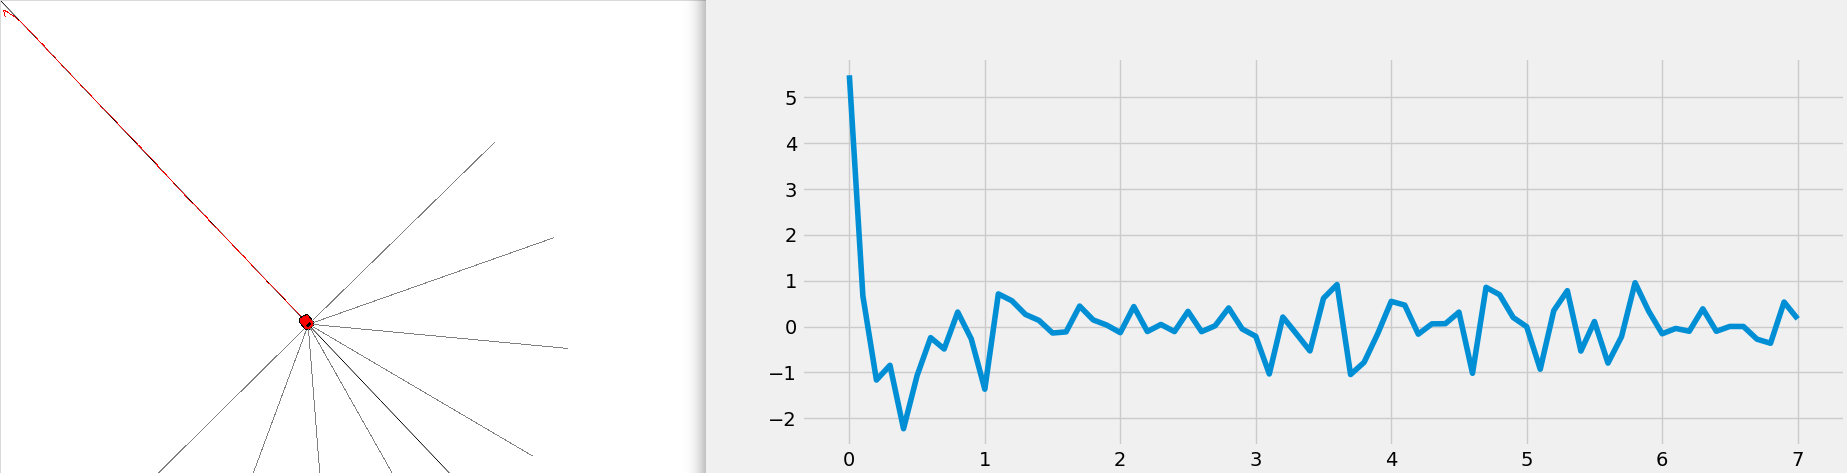
\includegraphics[width=.9\linewidth]{../doc-images/linea_grafica.png}
\captionof{figure}{Ejemplo del robot siguiendo una línea recta, con su gráfica de error adjunta}


\subsection{Otras consideraciones al seguimiento de la línea}
\label{sec-1-3}
Otro de los cambios que realizamos fue la reacción del robot cuando pierde la línea. En este caso, en
lugar de parar el robot, distinguimos entre dos situaciones:
\begin{enumerate}
\item Si el robot acaba de iniciarse, es decir, nunca ha encontrado una línea, comienza a describir una espiral hasta que la encuentra.
\item Si el robot ya se encontraba en una línea, entonces sabemos que la línea no puede estar lejos, por lo que se para y rota hasta que la encuentra.
\end{enumerate}


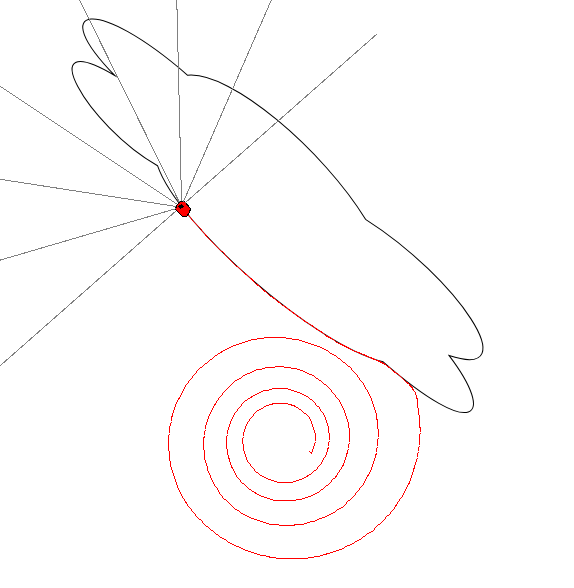
\includegraphics[width=.9\linewidth]{../doc-images/espiral_nube.png}
\captionof{figure}{Caso 1: El robot describe una espiral hasta que encuentra la línea}


\subsection{Límites del sistema}
\label{sec-1-4}
El control no funciona todas las veces cuando se encuentra una curva muy cerrada, puesto que en algunos
casos detecta las dos líneas como una sola y calcula el centro de esta línea virtual. Además, si encuentra
la línea de forma perpendicular a su trayectoria, necesita varios intentos, como se muestra en la siguiente
imagen


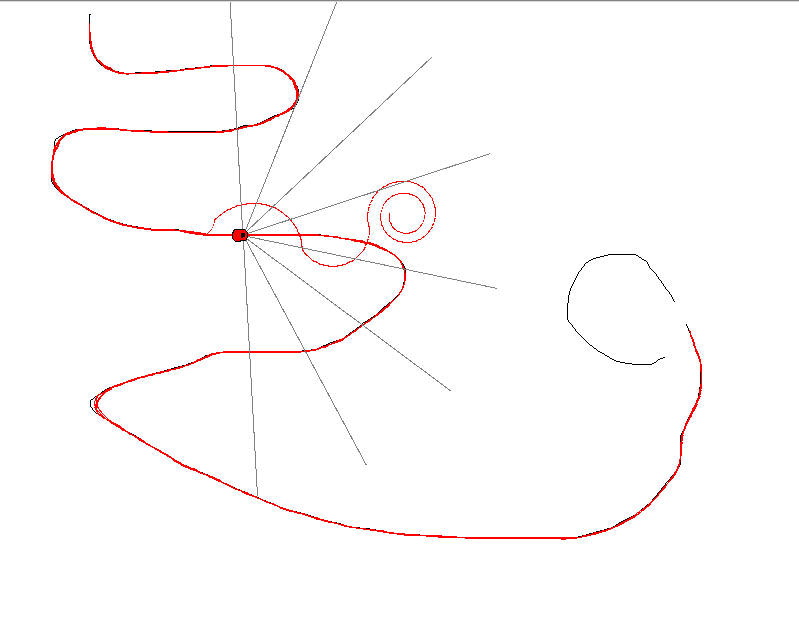
\includegraphics[width=.9\linewidth]{../doc-images/perpendicular.png}
\captionof{figure}{Error para seguir la línea cuando se encuentra de forma perpendicular}

\subsection{Pruebas realizadas para el seguimiento de la línea}
\label{sec-1-5}
Además de los ya mostrados, a continuación se muestran los recorridos del robot en diferentes mapas.

\begin{center}
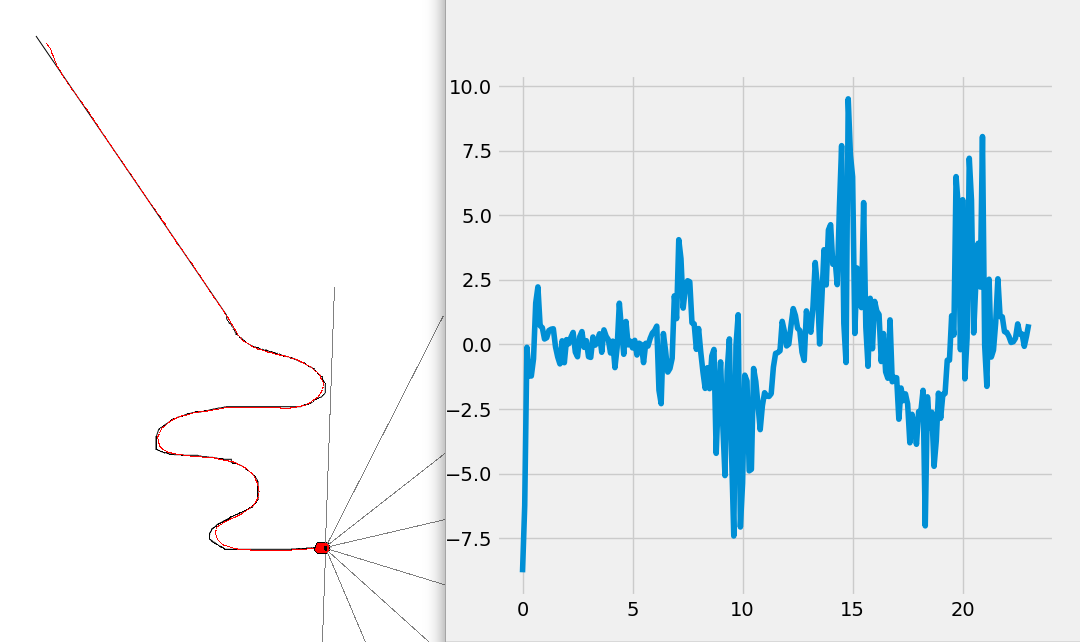
\includegraphics[width=.9\linewidth]{../doc-images/circuito1_grafica.png}
\captionof{figure}{Recorrido por el circuito inicial, con gráfica de error}


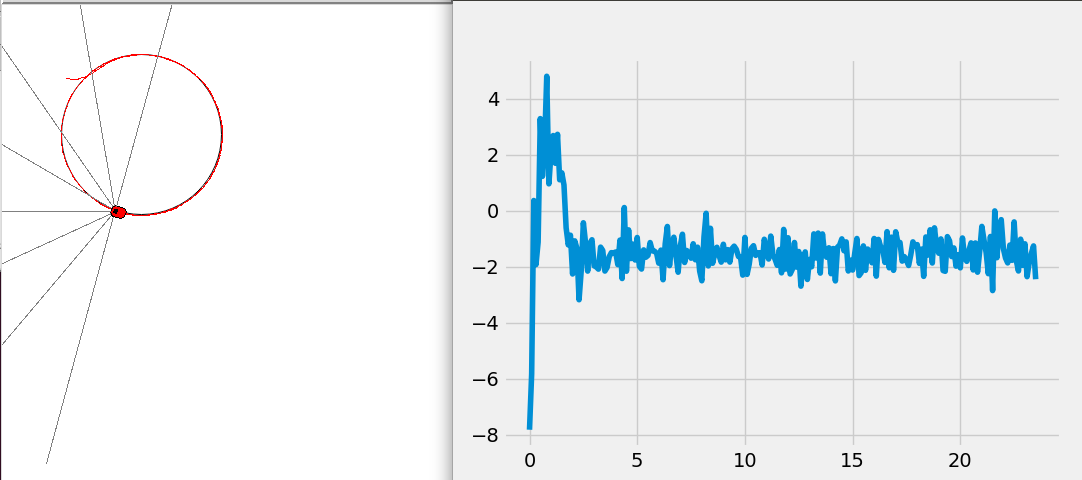
\includegraphics[width=.9\linewidth]{../doc-images/circulo_grafica.png}
\captionof{figure}{Recorrido por una circunferencia, con gráfica de error}


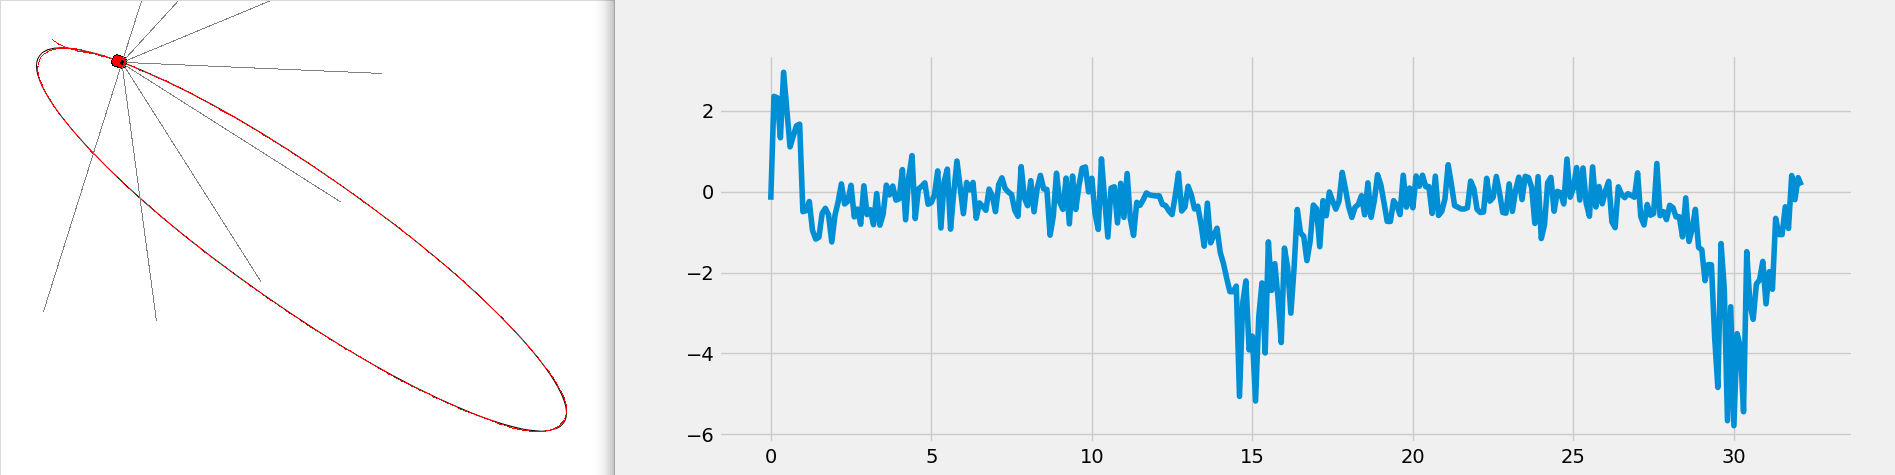
\includegraphics[width=.9\linewidth]{../doc-images/espiral1_grafica.png}
\captionof{figure}{Recorrido por una elipse no muy excéntrica, con gráfica de error}


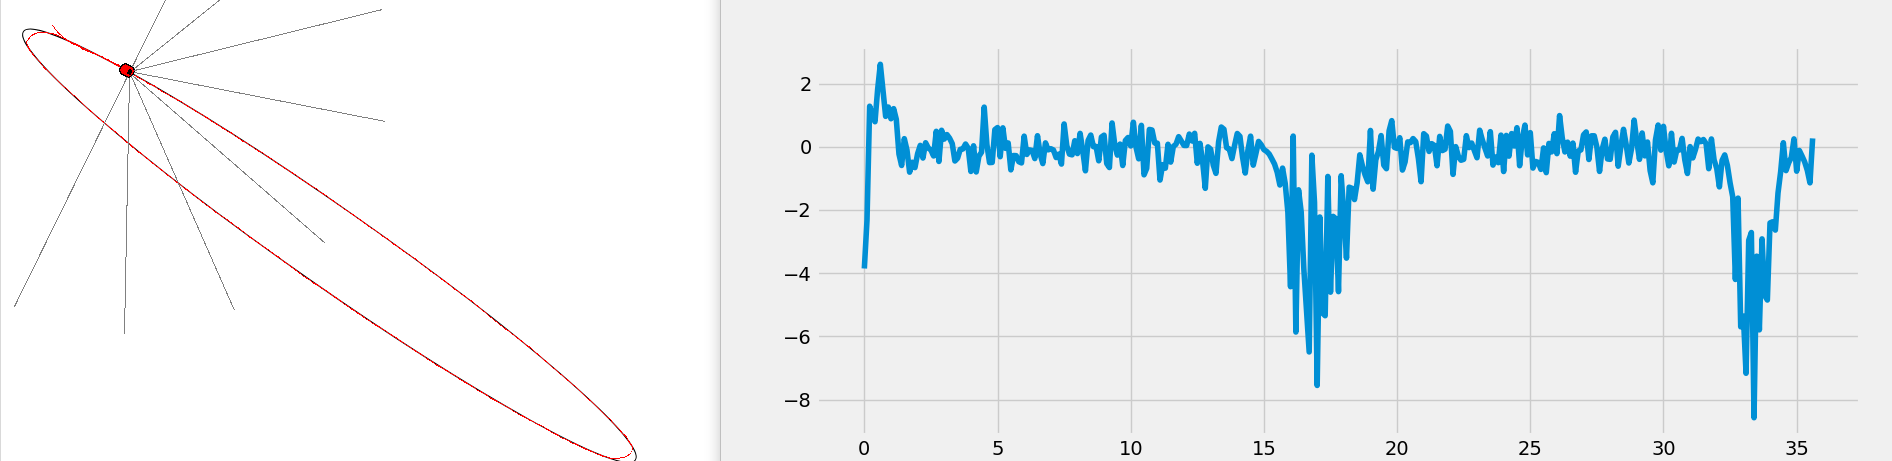
\includegraphics[width=.9\linewidth]{../doc-images/espiral2_grafica.png}
\captionof{figure}{Recorrido por una elipse de mayor exentricidad, con gráfica de error}


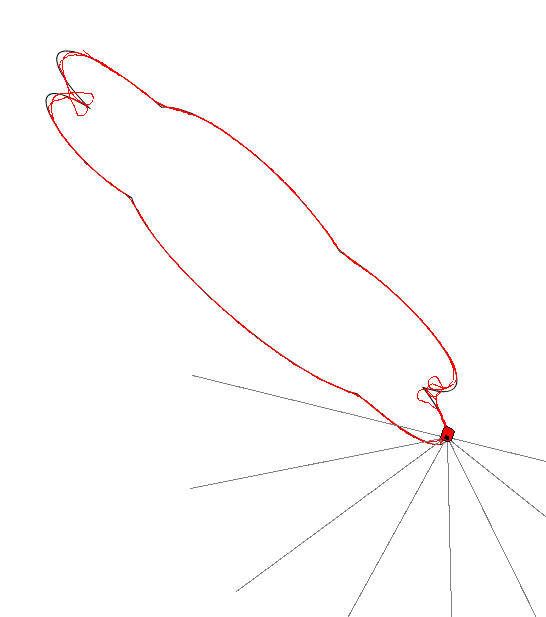
\includegraphics[width=.9\linewidth]{../doc-images/nube.png}
\captionof{figure}{Recorrido por una figura como una nube, con errores en las curvas más cerradas}


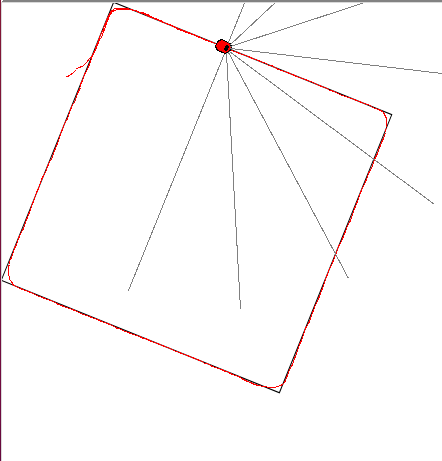
\includegraphics[width=.9\linewidth]{../doc-images/cuadrado.png}
\captionof{figure}{Recorrido por un cuadrado}

\end{center}
\pagebreak
\section{Esquive de obstáculos}
\label{sec-2}
Para detectar y esquivar obstáculos utilizamos los sonar del robot. Diferenciamos entre dos estados:
seguir una pared y girar una esquina cóncava con respecto al robot.

\subsection{Seguir una pared}
\label{sec-2-1}
Para seguir la pared, intenta mantener la distancia con la misma dentro de un rango, de esta manera,
si se detecta que la distancia es menor que un umbral, se gira para alejarse y viceversa cuando se
detecta una distancia mayor. A partir de la definición, se observa que este mismo estado sirve para
girar las esquinas convexas con respecto al robot, como las que se encuentra cuando rodea una caja
rectangular. Cuando se encuentra una pared de frente suponemos que se haya en una esquina cóncava,
como las que se puede encontrar cuando sigue las paredes por dentro de una habitación. En este caso,
pasa al siguiente estado

\subsection{Rodear una esquina}
\label{sec-2-2}
Tal y como está hecho el programa, el robot gira siempre en el mismo sentido, por lo que siempre podemos
suponer que tiene la pared al mismo lado y, por lo tanto, siempre que se encuentra una pared de frente
gira en sentido contrario hasta que detecta que la distancia frontal con la pared es suficientemente grande.
% Emacs 25.1.1 (Org mode 8.2.10)
\end{document}
